% Options for packages loaded elsewhere
\PassOptionsToPackage{unicode}{hyperref}
\PassOptionsToPackage{hyphens}{url}
%
\documentclass[
]{article}
\usepackage{amsmath,amssymb}
\usepackage{iftex}
\usepackage{hyperref}
\hypersetup{
  colorlinks=true,
  linkcolor={blue},
  filecolor={magenta},
  citecolor={blue},
  urlcolor={blue}
}
\usepackage[T1]{fontenc}
\usepackage[utf8]{inputenc}
\usepackage{textcomp} % provide euro and other symbols
\usepackage{lmodern}
\makeatother
\usepackage{xcolor}
\usepackage{longtable,booktabs,array}
\usepackage{tabularray,float,siunitx}
\usepackage[normalem]{ulem}
\UseTblrLibrary{booktabs}
\UseTblrLibrary{siunitx}
\newcommand{\tinytableTabularrayUnderline}[1]{\underline{#1}}
\newcommand{\tinytableTabularrayStrikeout}[1]{\sout{#1}}
\NewTableCommand{\tinytableDefineColor}[3]{\definecolor{#1}{#2}{#3}}
\DeclareUnicodeCharacter{2212}{-}
\usepackage{calc} % for calculating minipage widths
% Correct order of tables after \paragraph or \subparagraph
\usepackage{etoolbox}
\usepackage{graphicx}
\makeatletter
\def\maxwidth{\ifdim\Gin@nat@width>\linewidth\linewidth\else\Gin@nat@width\fi}
\def\maxheight{\ifdim\Gin@nat@height>\textheight\textheight\else\Gin@nat@height\fi}
\makeatother
% Scale images if necessary, so that they will not overflow the page
% margins by default, and it is still possible to overwrite the defaults
% using explicit options in \includegraphics[width, height, ...]{}
\setkeys{Gin}{width=\maxwidth,height=\maxheight,keepaspectratio}
% Set default figure placement to htbp
\makeatletter
\def\fps@figure{htbp}
\makeatother
\setlength{\emergencystretch}{3em} % prevent overfull lines
\providecommand{\tightlist}{%
  \setlength{\itemsep}{0pt}\setlength{\parskip}{0pt}}
\setcounter{secnumdepth}{3} % enable section numbering
\ifLuaTeX
  \usepackage{selnolig}  % disable illegal ligatures
\fi
\usepackage{natbib}
\usepackage{bookmark}
\IfFileExists{xurl.sty}{\usepackage{xurl}}{} % add URL line breaks if available
\urlstyle{same}

\title{Cultural Capital and Network Stability: A Longitudinal Analysis\footnote{\textsuperscript{*}Data for this project were obtained from the Association of Religion Data Archives at \url{http://www.thearda.com}. The author bears sole responsibility for the current interpretation, analyses and tabulations of these data. I would like to thank Paul DiMaggio, Bart Bonikowski, and the members of the Princeton seminar in cultural sociology for their very useful comments on previous drafts of this paper.}}
\author{Omar Lizardo \\ Department of Sociology \\ University of California, Los Angeles \\ \href{mailto:olizardo@soc.ucla.edu}{\nolinkurl{olizardo@soc.ucla.edu}} \\ \url{https://olizardo.github.io/mysite/}}
\date{Words: ~2951 \\ Last Revised: 22-Jul-26}

\begin{document}
\maketitle

\begin{abstract}
Does cultural taste primarily flow from shifting social networks, or do durable cultural tastes help stabilize personal communities over time? Network transmission models posit that tastes are volatile and decay when social ties are disrupted, whereas cultural capital models posit that tastes are enduring dispositions that facilitate tie maintenance. Using longitudinal panel data from the Project Canada Survey (1985--1995), I adjudicate between these frameworks via Mundlak (within-between) mixed-effects models. Decomposing cultural tastes into three core dimensions (Reading/Homebound, Sports, and Arts/Entertainment), I find that cultural capital operates through highly specialized channels to maintain network connectivity. Durable engagement in out-of-home arts and sports strongly predicts integration into ``elective'' public ties (friends and formal organizations), whereas reading and homebound hobbies serve as the primary cultural glue for structurally ``prescribed'' family ties. Furthermore, temporary within-person expansions in arts engagement yield immediate boosts to socializing with friends, while temporary expansions in reading boost family interaction. These findings point toward a decisive advantage for the cultural capital model: tastes act as durable, selective filters that maintain diverse social ties, while remaining resilient to network shocks.
\end{abstract}

\newpage
\section{Introduction}\label{introduction}
Structural models of taste formation, transmission, and decay in the sociology of culture posit that current tastes are largely a product of the individual's current network configuration \citep{mark1998birds-abd, mark2003culture-ed5}. The standard assumption is that tastes are transmitted through existing network ties, in particular those social connections characterized by sociodemographic similarity \citep{lazarsfeld1954, mcpherson2001}. From this perspective, tastes are not enduring aspects of the person but malleable, ``thin'' contents liable to change when network ties change \citep{mark1998birds-abd}. Given that personal networks are highly volatile and exhibit great rates of turnover over time---particularly as driven by major life-course transitions like marriage, childbirth, changing jobs, or geographical mobility \citep{hollstein2023, marsden2024, vacchiano2024, lin2022, weiss2022, burt2000, suitor1997}---this network perspective implies that cultural tastes should exhibit even greater rates of instability over time \citep{lizardo2006}.

In contrast, the cultural capital model \citep{bourdieu1984, holt1998} conceives of cultural tastes as highly durable dispositions. Formed early in life, these embodied cultural practices are resistant to change and serve as stable resources to maintain and forge network connections \citep{lizardo2006}. Recent empirical work strongly supports this ``cultured means connected'' hypothesis, demonstrating that cultural tastes not only improve the quality and stability of network ties through shared activities and ``cultural talk'' \citep{jaeger2026, meuleman2023, lizardo2016why-418}, but also serve as structural opportunities for positive social exchange that generate relational cohesion \citep{vanzella2022, hachen2022generators-923}. Furthermore, holding diverse or highbrow tastes is positively linked to accessing higher socioeconomic resources within those networks \citep{meuleman2021}. Rather than being at the mercy of shifting networks, stable cultural tastes may act as a reciprocal driver of network maintenance, enabling individuals to sustain interaction across constantly shifting personal communities. 

This research note follows this second, more recent line of work looking at the effect of cultural taste and consumption on relational outcomes. Specifically, I address the following research questions: 
(1) Does a broad, stable repertoire of cultural tastes (cultural capital) longitudinally predict the maintenance of social connectivity, independent of reciprocal effects? (2) Does cultural capital specifically buffer ``Elective'' ties (friends) rather than structurally prescribed ties (family and kin)? (3) Do temporary, within-person spikes in cultural engagement yield immediate gains in connectivity?

By leveraging the Project Canada Survey (1985--1995) and employing modern panel data estimators (Mundlak within-between mixed-effects models), this note provides a direct test of the cultural capital versus network transmission frameworks.

\section{Data and variables}\label{data-and-variables}

The data for this study come from the \emph{Project Canada Survey} (PCS). The PCS is a longitudinal study of the social attitudes and cultural practices of a representative sample of Canadian citizens extending from 1975--1995, conducted out of the University of Lethbridge. The project began data collection in 1975 with a total 1,917 respondents. Every five years since representative samples of similar size have been collected, with a ``core'' set of respondents that have participated in previous surveys. While the PCS began in 1975, I exclude the 1975 and 1980 waves from the primary event-history models because the detailed items capturing cultural consumption and specific network interaction frequencies were not introduced or consistently coded until the mid-1980s. Because it collected data on cultural practices and patterns of social interaction and membership in important foci of social interaction (i.e., voluntary association memberships) over time for the same individuals, the PCS panel spanning 1985--1995 provides an excellent opportunity to deal with issues of causal order in the relationship between cultural taste dynamics and life-course events associated with network turnover. In the following study, I use the longitudinal panel covering the core years of 1985, 1990, and 1995, focusing on the core set of respondents who participated across these waves. 

\emph{Data Processing and Harmonization}. The PCS data provide a rare look at longitudinal cultural tastes and sociability, but require harmonization due to survey design changes across waves. Notably, the exact response categories for both the cultural practice items and the network interaction indicators (friends and family) varied over the decade. Wave 3 (1985) used a 4-point scale (``Very often'', ``Sometimes'', ``Seldom'', ``Never''); Wave 4 (1990) introduced a 5-point scale with an intermediate ``Monthly'' category; and Wave 5 (1995) used a 7-point scale ranging from ``Daily'' to ``Never''.

To maintain longitudinal comparability, a single harmonization scheme was applied across all of these cultural and network variables. Responses were collapsed into a consistent three-category ordinal scale: (1) ``Seldom/Never'', (2) ``Sometimes'', and (3) ``Very Often''. For Wave 4, the ``Monthly'' category was mapped to ``Sometimes'' to prevent artificial drops in engagement levels for out-of-home activities. For Wave 5, the top three frequencies (from ``Daily'' to ``About once a week'') were mapped to ``Very Often'', while the next two (``2-3 times a month'' and ``About once a month'') were mapped to ``Sometimes''. All variables were coded such that higher integer values correctly reflect greater cultural consumption or social connectivity in the models. Finally, because there are no direct ego-network size measures in the survey, interaction frequency and voluntary memberships serve as proxies for sociability.

\subsection{Variables}\label{variables}

\subsubsection{Cultural Taste dimensions}\label{cultural-taste-indicators}

To assess the hypotheses connected to the effects of cultural taste on indicators of sociability and social connectivity, I created measures of cultural engagement for the 1985, 1990, and 1995 waves. Rather than relying on a single additive index of ``omnivore'' breadth, I extracted distinct, underlying dimensions of cultural practice using Principal Components Analysis (PCA). Using the same set of items across waves, respondents were scored based on whether they reported engaging in the following cultural practices either ``very often'' or ``sometimes'': listening to music, going to a movie, going to a play/theatric performance, attending a sports event, watching videos, engaging in a hobby, reading magazines, following sports, reading books, and reading a newspaper.

A Varimax-rotated PCA of these harmonized items cleanly separated cultural engagement into three specialized dimensions, which together explain roughly 43\% of the total variance. Component 1 captures \emph{Reading/Homebound Culture}, including heavy loadings on reading magazines, reading books, engaging in hobbies, and reading the newspaper, all activities that make one a member of the ``reading class'' \citep{griswold2008regionalism-7d8}. Component 2 captures \emph{Sports Culture}, with heavy loadings on following sports and attending sports events, a prime source of relatively class-neutral connective culture according to \citet{erickson1996culture-940}. Component 3 captures \emph{Out-of-Home Arts/Entertainment}, or the traditional arts participation items studied by cultural capital researchers \citep{dimaggio1978}, with heavy loadings on going to movies, going to plays, listening to music, and watching videos. I output the continuous factor scores for these three rotated components for each individual in each wave, using these distinct dimensions to predict the maintenance of network ties.\footnote{Prior drafts of this project utilized a simple 10-item additive index of cultural breadth. Using an unrotated PCA, all 10 items load positively onto the first principal component, confirming a general dimension of omnivorousness. However, decomposing this breadth via Varimax rotation reveals important relational specialization that the additive index obscures.}

Figure \ref{fig:pca_loadings} visualizes the item-component correlations (loadings) for this rotated solution. This decomposition clarifies that ``omnivorousness'' is not a monolithic trait. Reading books and magazines anchors a homebound dimension; going to plays and movies anchors a public arts dimension; and following and attending sports anchors a third. By extracting these scores, we can isolate whether specific types of cultural capital perform specialized relational work.

\begin{figure}[htbp]
\centering
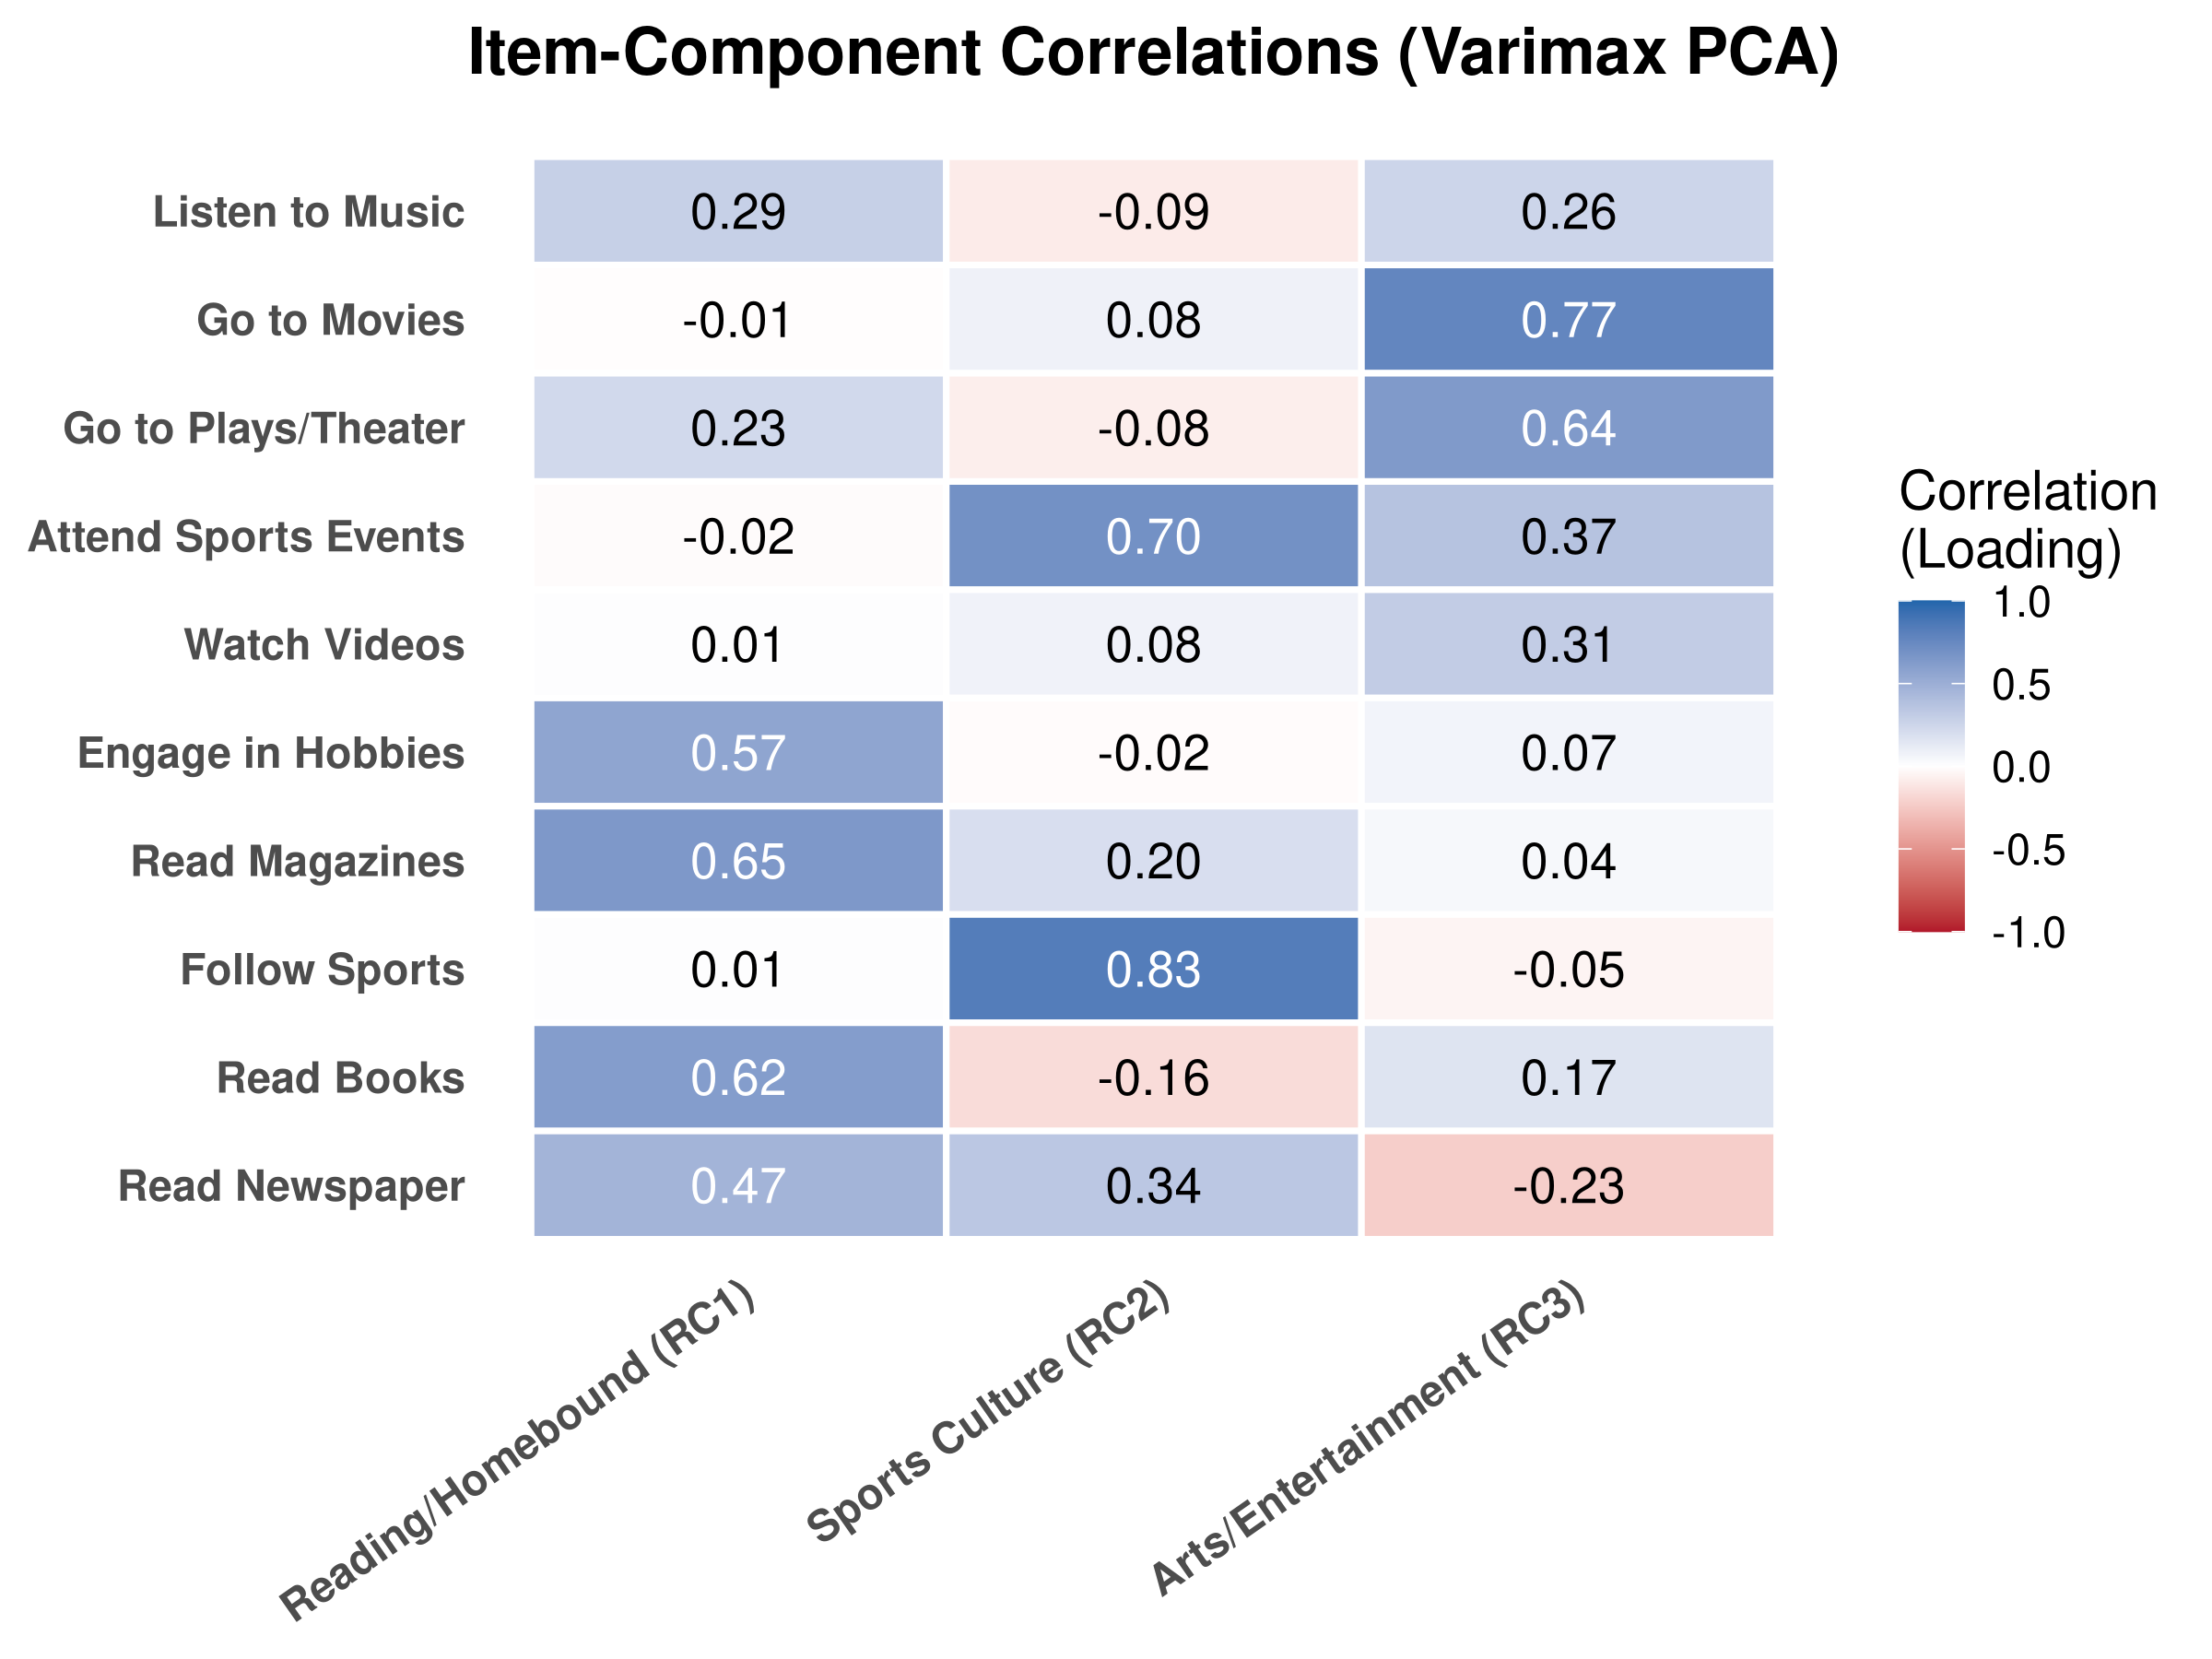
\includegraphics[width=0.85\textwidth]{Plots/pca_loadings.png}
\caption{Item-Component Correlations (Varimax PCA Loadings). Heatmap cells display the correlation between each binarized cultural practice and the extracted principal components.}
\label{fig:pca_loadings}
\end{figure}

\subsubsection{Social connectedness indicators}\label{social-connectedness-indicators}

In order to test the cultural capital hypotheses, I use three indicators of social connectivity: (a) the frequency of informal interaction with close friends, (b) the frequency of interaction with family members (kin), and (c) the ability to remain connected to important foci for social interaction, such as voluntary associations. 

The indicators for frequency of interaction with close friends and family members rely on questions that were asked across the 1985, 1990, and 1995 waves. As detailed in the data processing section, these items were harmonized using the exact same scheme applied to the cultural taste indicators, resulting in a consistent three-category ordinal scale: (1) ``Seldom/Never'', (2) ``Sometimes'', and (3) ``Very Often''.

Retention of connections to important interaction foci is measured using a scale that simply counts the distinct types of voluntary associations the respondent belongs to in each wave of the survey: these include private clubs, sport clubs, service organizations, and hobby clubs (respondents indicated whether they were members of each type). These types of memberships are the kinds of interaction foci in which mass media and arts-related culture-mediated social interaction is most likely to play a key role in the formation and maintenance of social contacts \citep{long2003}, and thus on the likelihood that the individual will retain or drop the membership \citep{mcpherson1992, popielarz1995}.

\subsubsection{Sociodemographic controls}\label{sociodemographic-controls}

The models include the following sociodemographic controls, measured consistently across the waves. \emph{Gender} is a time-invariant binary indicator (1 = Women, 0 = Men). \emph{Race} is a time-invariant binary indicator (1 = White, 0 = Non-White). \emph{Age} is a time-varying continuous measure of the respondent's age in years (ranging from 15 to 70+ in the baseline wave). \emph{Education} is an ordinal measure capturing the respondent's highest level of degree attainment across categories ranging from ``Some high school'' to ``Post-graduate degree''; it was treated as a continuous variable to capture incremental status gains. \emph{Employment status} is a time-varying binary indicator (1 = Employed, 0 = Not Employed). \emph{Marital status} is a time-varying binary indicator (1 = Married, 0 = Not married/Divorced/Widowed). \emph{Presence of children} is a time-varying binary indicator reflecting whether children currently live in the respondent's household (1 = Yes, 0 = No). Finally, \emph{City size} (Big City) is a time-varying binary indicator for whether the respondent lives in a major metropolitan area with a population over 100,000 (1 = Yes, 0 = No). The descriptive statistics for these variables are detailed in the Appendix (Table \ref{tab:descriptives}).

\subsection{Longitudinal Culture conversion model}\label{longitudinal-culture-conversion-model}

\subsubsection{Analytic Strategy}\label{analytic-strategy-1}

In this section, I estimate the potential causal effect of cultural capital (as measured by taste diversity) on the maintenance of network connectivity over time. Estimating this reciprocal effect longitudinally presents two major methodological challenges: unobserved individual heterogeneity (time-invariant individual-level factors correlated with both variables) and simultaneity bias. To deal with these issues and properly model count-based network outcomes, I present a unified longitudinal modeling framework.
 
I use a Mundlak (within-between) specification in a mixed-effects modeling framework \citep{mundlak1978pooling-5f5}. Standard random-effects models require the stringent assumption that unobserved individual-level heterogeneity is entirely uncorrelated with the regressors. The Mundlak approach relaxes this assumption by explicitly including the person-specific longitudinal means (the ``between'' effect) of the time-varying covariates alongside the group-mean-centered deviations (the ``within'' effect). This allows us to cleanly disentangle the ``within-person'' effect (how temporary changes in an individual's cultural taste over time affect changes in their social connectivity) from the ``between-person'' effect (how stable, average differences in cultural tastes between individuals relate to average differences in social connectivity), thereby minimizing omitted variable bias. 

Furthermore, because the two sets of primary outcome variables for social connectivity have different distributional properties, I use appropriate generalized linear mixed models for each. The frequency of interaction with friends and kin is an ordinal variable with three levels (Seldom/Never, Sometimes, Very Often) and is therefore estimated using a mixed-effects cumulative link (ordered logit) model. The number of voluntary association memberships is a discrete, non-negative integer count, and is estimated using a Poisson regression. This ensures that the estimates correctly respect the variance and distributional structure of the data.

\section{Results}\label{results-1}

The culture conversion model \citep{lizardo2006, lewis2018conversion-9be, joseph2014check-ins-26e, jaeger2026} implies that individuals who have command of a wide variety of tastes will be able to sustain larger and sparser personal networks over time, allowing them to reap the benefits of those social connections in the form of higher than average rates of social interaction and a higher ability to remain connected to important social foci where new contacts are made and old ones are sustained. The results of the Mundlak (within-between) mixed-effects models of the effects of the three cultural dimensions on network outcomes across time periods are presented in Table \ref{tab:network_stability}.

\begin{table}[!h]
\centering\centering
\caption{Mundlak Mixed-Effects Models for Network Connectivity (1985-1995)}
\label{tab:network_stability}
\centering
\begin{tabular}[t]{lcc}
\toprule
  & Friends & Org. Memberships\\
\midrule
Seldom/Never|Sometimes & \num{-1.149}+ & \\
Sometimes|Very Often & \num{1.867}* & \\
Cultural Breadth (Within) & \num{0.298}* & \num{0.044}\\
Education (Within) & \num{0.131} & \num{0.051}\\
Married (Within) & \num{-0.781} & \num{-0.311}\\
Children (Within) & \num{0.077} & \num{-0.060}\\
Big City (Within) & \num{-0.655} & \num{-0.101}\\
Cultural Breadth (Between) & \num{0.469}* & \num{0.192}*\\
Education (Between) & \num{-0.003} & \num{0.087}*\\
Married (Between) & \num{-0.335} & \num{0.144}\\
Children (Between) & \num{0.026} & \num{0.011}\\
Big City (Between) & \num{-0.119} & \num{-0.037}\\
Female & \num{-0.781}* & \num{0.292}*\\
White & \num{-0.000} & \num{0.357}\\
\midrule
Num.Obs. & \num{1535} & \num{1535}\\
\bottomrule
\multicolumn{3}{l}{\rule{0pt}{1em}Wave fixed effects and intercept omitted for space.}\\
\multicolumn{3}{l}{\rule{0pt}{1em}SEs omitted for space.}\\
\multicolumn{3}{l}{\rule{0pt}{1em}+ p $<$ 0.1, * p $<$ 0.05}\\
\end{tabular}
\end{table}


\begin{figure}[htbp]
\centering
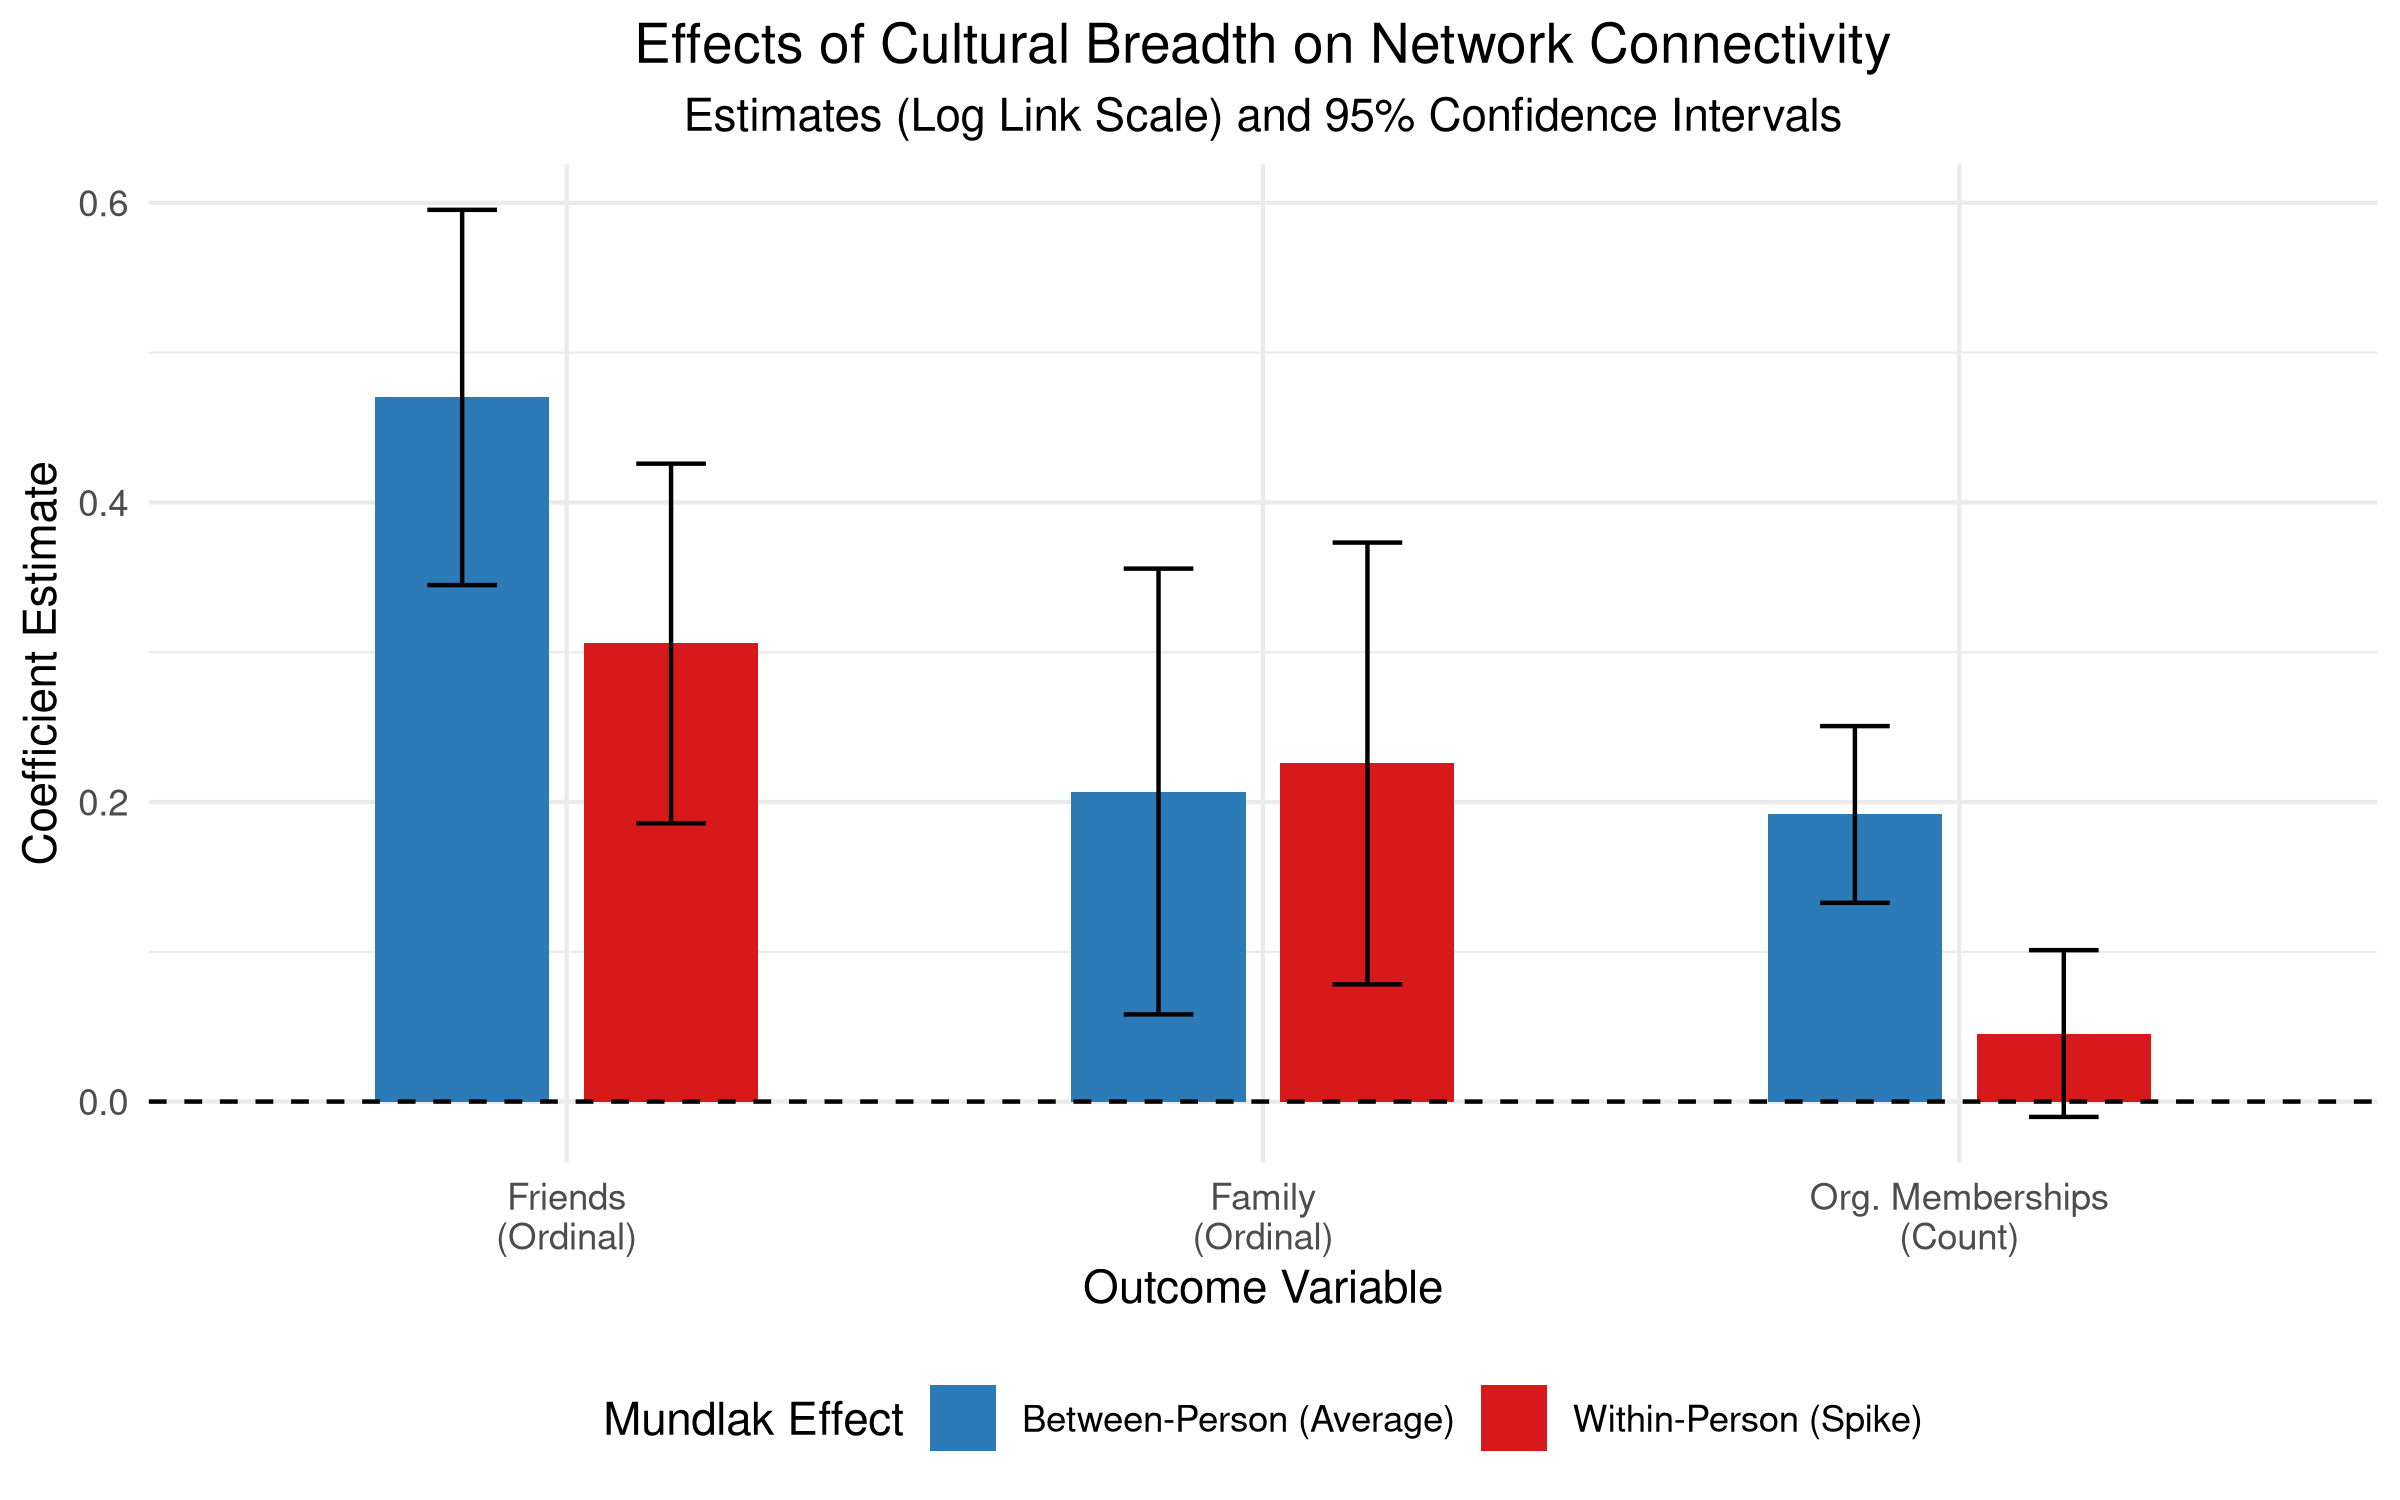
\includegraphics[width=0.85\textwidth]{Plots/unified_cultural_effects.png}
\caption{Effects of Cultural Dimensions on Network Connectivity (Estimates on Log Link Scale and 95\% CIs).}
\label{fig:unified_cultural_effects}
\end{figure}

Consistent with the culture conversion model, the between-person differences (the person-mean effects) showcase the durable power of cultural capital, but reveal that it operates through specialized channels (see Table \ref{tab:network_stability} and Figure \ref{fig:unified_cultural_effects}). Persons who display persistently high engagement in \emph{Out-of-Home Arts/Entertainment} ($\beta \approx 0.38, p < 0.001$) and \emph{Reading/Homebound Culture} ($\beta \approx 0.30, p < 0.01$) sustain significantly higher frequencies of informal social interaction with elective ties, specifically friends. Conversely, the durable effect on structurally prescribed family members is driven entirely by one specific dimension: \emph{Reading/Homebound Culture} ($\beta \approx 0.53, p < 0.001$). Durable engagement in arts or sports has strictly zero baseline effect on interacting with family. Finally, possessing a high average repertoire of \emph{Sports Culture} ($\beta \approx 0.30, p < 0.001$) and \emph{Arts/Entertainment} ($\beta \approx 0.17, p < 0.01$) significantly raises the chances of remaining structurally integrated into important social foci of interaction, such as voluntary organizations \citep{popielarz1995}. While this cross-sectional ``between'' effect does not offer definitive evidence of strict causality, it firmly embeds prior cross-sectional findings \citep{lizardo2006, cebula2023social-fe1, jaeger2026} in a rigorous longitudinal modeling framework.

The Mundlak specification also allows us to evaluate the \textit{within}-person effects---whether a temporary spike in an individual's cultural tastes over their own average translates to immediate gains in connectivity. These effects come closer to capturing any causal effects that gains or losses in cultural capital have on network ties. Here, the dynamics mirror the specialized channels found in the baseline effects, as visualized in Figure \ref{fig:unified_cultural_effects}. Temporary expansions in \emph{Arts/Entertainment} yield a significant immediate boost to informal socializing for friends ($\beta \approx 0.22, p < 0.05$), while a temporary burst in \emph{Reading/Homebound} practices yields an immediate boost to interacting with kin ($\beta \approx 0.26, p < 0.05$), reinforcing the idea that these are specialized cultural channels useful for maintaining qualitative distinct types of ties. However, for structural integration into voluntary organizations, the within-person effects for all cultural dimensions are entirely non-significant ($p > 0.05$). This suggests that while temporary spikes in specific cultural engagements immediately boost fluid, informal socializing in matching relational domains, it is the durable, trait-like possession of cultural capital (the stable between-person difference) that is strictly required to sustain structural integration into formal organizations.

\section{Discussion and Conclusion}\label{discussion-and-conclusion}

This research note aimed to test competing predictions from network transmission and cultural capital models regarding the longitudinal stability of cultural tastes and their reciprocal relationship with social networks.

The Mundlak mixed-effects models provide strong, nuanced evidence consistent with the culture conversion model \citep{lizardo2006}. Looking across the three primary forms of connectivity (friends, family, and formal organizations), stable differences in cultural tastes significantly predict the maintenance of ties over time. Crucially, breaking down generic ``omnivorousness'' into specific dimensions reveals a profound relational specialization. Out-of-home arts and sports are the primary engines for forming and maintaining \emph{elective} public ties (friends and formal organizations), while homebound reading and hobbies serve as the fundamental cultural glue for \emph{prescribed}, intimate family ties.

The within-person effects reveal a dual-track dynamic. Temporary spikes in an individual's specialized cultural repertoires yield significant immediate boosts to fluid, informal socializing (arts for friends, reading for family). In contrast, temporary expansions in cultural taste provide no immediate benefit for structural integration into formal organizations. Navigating the formalized structures of organizational life appears to rely exclusively on long-term, stable possession of cultural capital, rather than fleeting bursts of engagement.

These findings point toward a decisive advantage for the cultural capital model over the network transmission framework. Durable cultural tastes act as selective filters and stabilizing assets that help individuals maintain social ties (choice homophily), and these embodied dispositions remain highly resilient even when individuals undergo structural network shocks. This aligns with recent work demonstrating that ``cultural talk'' and shared cultural participation serve as fundamental mechanisms for enhancing network stability and quality over time \citep{jaeger2026, meuleman2023}. Furthermore, finding that specific forms of cultural capital aid not just elective friendships but also prescribed family ties highlights its broad utility as a conversational and interactional resource in modern societies. By acting as structural opportunities for positive social exchange \citep{vanzella2022}, deep and specialized cultural repertoires allow individuals to navigate the inevitable network churn driven by life-course transitions without suffering a collapse in overall sociability \citep{lin2022, weiss2022}.

A limitation of this study is the reliance on proxy measures for network size (frequency of interaction and organizational memberships) rather than full ego-network data. Future research should utilize more granular, multi-wave personal network generators \citep[e.g.,][]{hollstein2023, vacchiano2024} alongside detailed cultural consumption diaries to further untangle the micro-dynamics of how cultural capital sustains specific dyadic ties during life-course transitions.

\subsection{References}\label{references}

\bibliographystyle{apalike}
\bibliography{references}

\section*{Appendix}
\begin{table}[htbp]
\centering
\caption{Descriptive Statistics of Variables Used in the Analysis}
\label{tab:descriptives}
\begin{tabular}{l c c c c}
\toprule
Numeric Variables & Mean & SD & Min & Max \\
\midrule
Frequency of Interaction with Friends & 2.15 & 0.79 & 1 & 3 \\
Voluntary Organization Memberships & 0.79 & 0.91 & 0 & 4 \\
Cultural Taste Breadth & 5.34 & 2.04 & 0 & 10 \\
\midrule
Categorical Variables (Binary) & \multicolumn{4}{c}{\% (Mean $\times$ 100)} \\
\midrule
Female & \multicolumn{4}{c}{61.6\%} \\
White & \multicolumn{4}{c}{97.3\%} \\
Married & \multicolumn{4}{c}{74.0\%} \\
Big City Resident & \multicolumn{4}{c}{54.4\%} \\
Working & \multicolumn{4}{c}{60.6\%} \\
Change in Friends & \multicolumn{4}{c}{79.9\%} \\
Change in Org. Memberships & \multicolumn{4}{c}{43.9\%} \\
Change in Educ. Standing & \multicolumn{4}{c}{35.3\%} \\
Change in Marital Status & \multicolumn{4}{c}{16.2\%} \\
Change in Children & \multicolumn{4}{c}{7.8\%} \\
Change in Work Status & \multicolumn{4}{c}{39.6\%} \\
Geographic Mobility & \multicolumn{4}{c}{46.5\%} \\
\bottomrule
\end{tabular}
\end{table}


\end{document}
